\documentclass{egpubl}
\usepackage{wait}

\ConferencePaper      % uncomment for (final) Conference Paper

\title[Fat Curves]{Fat Curves -- A title which is much too long to
                   serve as running head}

\author[Yao et al]
       {Chris Yao,$^1$\thanks{On leave from Suzhou Institute of Silk Textile Technology,
        P.R. China Since July 1988.}
        Anton Notherone$^2$ and
        Jeremy Rokne$^1$
        \\
        $^1$ Department of Computer Science, The University of Calgary, Calgary,
             Alberta, Canada\\
        $^2$ Another Department to illustrate the use in papers from authors
             with different affiliations
       }

%for including postscript figures
\usepackage[dvips]{graphicx}
% \usepackage[dvips,draft]{graphicx}% replace PS figure by framed file name

\PrintedOrElectronic

% prepare for electronic version of your document
\usepackage{t1enc,dfadobe}

% For backwards compatibility to old LaTeX type font selection.
% Uncomment if your document adheres to LaTeX2e recommendations.
\let\rm=\rmfamily    \let\sf=\sffamily    \let\tt=\ttfamily
\let\it=\itshape     \let\sl=\slshape     \let\sc=\scshape
\let\bf=\bfseries

% if the Editors-in-Chief have given you the data, you may uncomment
% the following five lines and insert it here
%
% \volume{22}   % the volume in which the issue will be published;
% \issue{3}     % the issue number of the publication
% \pStartPage{???}      % set starting page


\begin{document}

\maketitle

\begin{abstract}
Fat curves in two-dimensional Euclidean space are discussed. Previous
work on fat curves is reviewed and a new definition is given for a fat
curve having a smooth axis. The joining of two fat curves is discussed
and a technique for scan-converting fat curves is presented.

\begin{classification} % according to http://www.acm.org/class/1998/
\CCScat{I.3.3}{Computer Graphics}{Line and Curve Generation}
\end{classification}

\end{abstract}

\section{Introduction}

In computer graphics it is frequently desirable to represent a curve or
the outline of an object as ``thick'' or a ``fat'' curve. This is
particularly true for high-resolution graphics devices where curves
represented by a chain of single pixels are too faint or where for
aesthetic reasons the curve should have a fixed non-zero width. The
definition of such objects pose particular geometric problems.
Implementing the objects in terms of raster graphics similarly
introduces further problems in the scan-conversion process.

If we look to standard references on algorithms for computer graphics
such as Pavlides\cite{yll} then we do not find the fat line or curve concept.
In fact there are only two fundamental concepts considered by
Pavlides\cite{yll}: a thin curve with an orientation-dependent average width
ranging from $1/\sqrt{2}$ pixels to 1 pixel and a full region. Fat
curves are subsumed under the full region concept and no consideration
is given to the particular problems encountered in dealing with them.

We want here only show a possible citation, such as the typical citation of
the Foley et al. book \cite{FolDamFeiHug.etal93} or a well known paper on ray
tracing of volumetric dataset \cite{Lev90}. Fat lines are discussed in
Bresenham under the concept of \emph{Widelines\/} and he poses a number of
questions relating to this concept. A fundamental question is how the fat
lines are terminated and what the assumptions are when such lines are joined
at decreasing angles. To quote Bresenham:
%
\begin{quote}
  Is \emph{Wideline\/} a consistent concept, or is it a poorly specified and
  incompletely defined attempt to set up an implicit but fuzzily understood
  reference model of areas in contrast to lines? \ What is the shape of
  wideline ends? Is line width a geometric property in our original modeling
  co-ordinate space, or is such thickness only a picture-rendering cosmetic
  attribute akin to pseudo-pen size in final raster space? How should
  projective transformations affect \emph{Widelines}? If width is a geometric
  attribute, what is the implied boundary definition?
\end{quote}
In this paper we discuss some of the problems posed by Bresenham and we
suggest solutions both in the underlying geometric setting and in the raster
plane. We first give a precise definition of a fat line or curve as a
continuous geometric object. Then, using this definition, we develop new
algorithms implementing scan-conversion for such curves.

In the next section we survey previous definitions of fat lines concluding
with the specific problems that we attempt to solve in this paper. In
Section~\ref{sec:digErr} we consider the analytic definition of smooth fat
curves and we verify some simple properties. The problem of joining fat
curves is then dealt with and we introduce the concept of a piece-wise smooth
fat curve. Finally we give a method for the scan-conversion of the fat curves
we defined in the previous sections.


\section{Previous Work}

Fat lines are discussed in several recent papers, but here we cite papers
that have nothing in common with the \emph{fat line} topic
\cite{Lev90,FolHagNie93,PorDuf84,RonRos96}. The concept is also used by
several advanced workstations (see for example the IRIS User's Guide) and by
typesetting systems such as PostScript.

Perhaps the most relevant discussion is found in the paper by
Posch-Fellner.\cite{PosFel89}
They discuss an algorithm called options for double precision arithmetic. The
impact of using single precision arithmetic is demonstrated in Table~1. Even
when compiled with the double precision option, the program by Douglas
produces results which deviate significantly from those produced by others.
The formula used to calculate the squares of offset values presented in
Table~1 is as follows:
%
%Math
%
\begin{eqnarray*}
 \lambda\! &\!\!\!\! =\!\!\!\! & \frac{(x1\!*\!(x1\!\!-\!\!x2\!\!-\!\!x3)%
                                       \!+\!x2\!*\!x3\!+\!y1\!*\!%
                         (y1\!\!-\!\!y2\!-\!\!y3)\!+\!y2)}%
                    {(x2-x1)^2+(y2-y1)^2}\\
       x\! &\!\!\!\! =\!\!\!\! & x1+\lambda *(x2-x1)\\
       y\! &\!\!\!\! =\!\!\!\! & y1+\lambda *(y2-y1)\\
 \mbox{\rm dis}\! &\! =\! & (x3-x)^2+(y3-y)^2
\end{eqnarray*}
%
In a recent debate on the accuracy of floating point calculations, Huggins
stated that the arbitrary-precision arithmetic language `bc' could be used to
obtain precise results. We used this UNIX utility to calculate offset values
for points C and D. On the VAX 8200, SEQUENT SYMMETRY and SUN 3/60, bc
returned identical values for these points:
%
%Math
%
\[\mbox{
C: 28143.490838958534 \hskip 15pt
D: 28143.49083895834
}\]
%
Forrest (p. 721) pointed out the well known fact that floating point
calculations are still very much machine dependent. Machine dependency
exposed further problems, which could be treated as problems of
implementation but which are arguably more conceptual in nature as explained
in the following sections.

\subsection{Equidistant points from the anchor-floater line}

The algorithm is based on the assumption that lines may be subdivided in an
unambiguous manner using the maximum perpendicular offset. To our knowledge,
the problem of two or more points being equidistant from the anchor-floater
line has never been considered. Indeed, we only became conscious of this
possibility when the same program yielded different results on ICL 3980 and
SUN 3/60 computers. A sample problem is illustrated in Figure~5. Points C and
D are equidistant from the anchor-floater line A--B. The inexact
representation of floating point numbers results in C being selected on SUN
workstations and D being selected on the ICL computer by the same program.
With double precision arithmetic, the errors are negligible but are
nevertheless sufficient to generate different results since published
programs tend to use either a ``greater than'' or ``less than'' condition.
GIMMS and the programs by Douglas and Wade select the first point from a set
of identical offsets. White's program selects the last. The results therefore
are variable and become dependent on the direction of digitising of lines.
If, on the other hand, we select a point from this set at random, the
procedure would become blatantly arbitrary. This problem poses other
implications, which we will now examine in greater detail.

%%%
%%% Figure 1
%%%
\begin{figure}[htb]
  \centering
  % the following command controls the width of the embedded PS file
  % (relative to the width of the current column)
  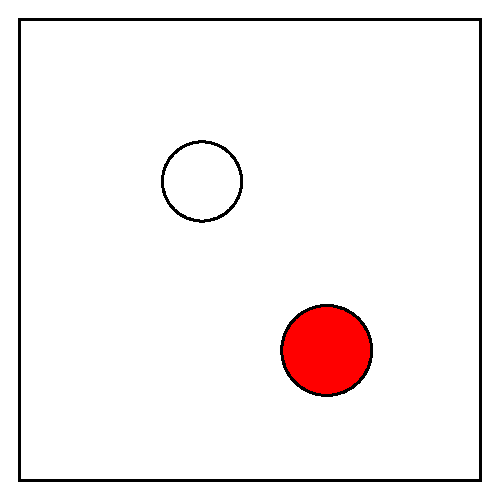
\includegraphics[width=.95\linewidth]{sample.eps}
  % replacing the above command with the one below will explicitly set
  % the bounding box of the PS figure to the rectangle (xl,yl),(xh,yh).
  % It will also prevent LaTeX from reading the PS file to determine
  % the bounding box (i.e., it will speed up the compilation process)
  % \includegraphics[width=.95\linewidth, bb=xl yl xh yh]{sampleFig.eps}
  \caption{\label{fig:firstExample}
           Here is a sample figure.}
\end{figure}


\section{Our proposal in detail}
\label{sec:propDet}

This section describes in detail our proposal, as graphically
shown also in Figure~\ref{fig:firstExample}, with a non-sense
text. Non-sense text follows text text text text text text text
text text texttext text text text texttext text text text texttext
text text text texttext text text text texttext text text text
texttext text text text texttext text text text texttext text text
text texttext text text text texttext text text text texttext text
text text texttext text text text texttext text text text texttext
text text text texttext text text text texttext text text text
texttext text text text texttext text text text texttext text text
text texttext text text text texttext text text text texttext text
text text text.


\section{Digitising Errors}
\label{sec:digErr}

Like most cartographic algorithms, the Douglas--Peucker algorithm does not
fully address the issue of digitising errors. When estimating truth values,
it is usually assumed that the true line (in this case the analogue line)
lies within the error band of the digitised line. This band is also known as
the Perkal epsilon band. In his review on issues relating to the accuracy of
spatial databases, Goodchild\cite{Lev90} indicated that researchers have
proposed uniform, normal and even bimodal distributions of error across this
band. This concept provides some basis for estimating the position of the
true line at locations between digitised points. Here, we are merely
concerned with the accuracy of digitised points. Whilst it is probable that
operators digitise points along high curvatures more carefully than at
intermediate positions, there is at present no sound basis for modelling the
distribution of error along the line. As in the Circular Map Accuracy
Standard, it is usual to assume a bivariate normal distribution of error when
estimating the position of the true point. In the context of line
simplification, absolute positional accuracy is less important than the
relative position of points describing the shape of features along the line.

The DoE/SDD boundary data contain some gross digitising errors. For example,
inlet X in Figure~2c does not feature on conventional Ordnance Survey
1:\,50\,000 maps of the area. The data are also not very accurate where
coastlines are convoluted. Even if we ignore these and other gross errors,
such as spikes, there will always be an element of random error in digitised
data. It is reasonable to assume that points digitised from 1:\,50\,000
source material may only be accurate to within $+/-5$ metres. This algorithm
does not lead to a substantial accumulation of rounding errors, hence the
numerical errors discussed earlier tend to be very small compared with
digitising errors.

For the purposes of our argument, it is unnecessary to undertake an
exhaustive evaluation of the consequences Douglas and Peucker have treated
overhangs and closed loops as different problems, and have used different
methods to cope with each case.

\subsection{Numerical Problems}

The FORTRAN programs by Douglas, White, and Wade use single precision REALS
when computing offsets (see results in Table~\ref{tab:calcPrec}). Whilst
double precision accuracy may be attained through the use of compiler
options, we are unsure whether previous research has been based on programs
compiled in this manner. Wade's program was so compiled for use in our
previous evaluations. Forrest stated that Ramshaw (1982) had to adopt
carefully tuned double and single precision floating point arithmetic to
compute the intersection of line segments whose end points were defined as
integers. Forrest exclaimed ``This is an object lesson to us all:
constructing geometric objects defined on a grid of points, requiring ten
bits for representation can lead to double precision floating point
arithmetic!''.

Most evaluative studies do not cite the co-ordinates in use. We do not know
whether the published test lines were in original digitiser co-ordinates or
whether they had been converted to geographic references. British National
Grid co-ordinates for the administrative boundaries of England, Scotland and
Wales (digitised by the Department of Environment (DoE) and Scottish
Development Department (SDD)) are input to one metre accuracy and require
seven decimal digits for representation if we include the northern islands of
Scotland. At the South West Universities Regional Computer Centre these
co-ordinates have been rounded to 10 metre resolution; even this requires six
decimal digits. Seamless cartographic files at continental and global scales
use much larger ranges of geographic co-ordinates.

\begin{table}[htb]
%\begin{center}
\small
\begin{tabular*}{\linewidth}%
{@{}l@{}l@{}c@{}c@{}c@{}l@{}}
\hline
Machine\,\,\, & Points &
\multicolumn{4}{@{}c}{\small Calculated squares of offset values}\\
 & & \multicolumn{2}{@{}c}{\small Single Precision}
& \multicolumn{2}{c@{}}{\small Double Precision}\\
\hline
\multicolumn{6}{@{}l}{ICL 3980} \\
& (C) & \multicolumn{2}{@{}c}{28199.351562500}
& \multicolumn{2}{c@{}}{28143.490838958}\\
 & (D) & \multicolumn{2}{@{}c}{28171.789062500}
& \multicolumn{2}{c@{}}{28143.490838961}\\
\multicolumn{6}{@{}l}{VAX 8200} \\
& (C) &\multicolumn{2}{@{}c}{28253.095703125}
&\multicolumn{2}{c@{}}{28143.490838958}\\
& (D) &\multicolumn{2}{@{}c}{28165.806640625}
&\multicolumn{2}{c@{}}{28143.490838958}\\
\multicolumn{6}{@{}l}{SEQUENT SYMMETRY}\\
& (C) &\multicolumn{2}{@{}c}{28145.100000000}
&\multicolumn{2}{c@{}}{28143.490838961}\\
& (D) &\multicolumn{2}{@{}c}{28145.100000000}
&\multicolumn{2}{c@{}}{28143.490838961}\\
\multicolumn{6}{@{}l}{SUN 3/60} \\
& (C) &\multicolumn{2}{@{}c}{28253.095703125}
&\multicolumn{2}{c@{}}{28143.490838961}\\
& (D) &\multicolumn{2}{@{}c}{28165.806640625}
&\multicolumn{2}{c@{}}{28143.490838961}\\
\hline
\\
\multicolumn{6}{@{}l}{\textsc{Notes}}\\[5pt]
\multicolumn{6}{@{}p{\linewidth}@{}}
{\emph{Offsets of points C and D from the anchor-floor line
A--B as calculated using Wade's program. Points A, B, C and D are shown in
Figure 5. The British National Grid coordinates (in metres) of the points
are as follows:}}\\[9pt]
\hline
Point A & \multicolumn{2}{l}{238040\,\, (x1)}  &
\multicolumn{2}{l}{205470\,\, (y1)}
&  \multicolumn{1}{c}{ANCHOR}\\
Point B  & \multicolumn{2}{l}{237890\,\, (x2)}
& \multicolumn{2}{l}{205040\,\, (y2)}
& \multicolumn{1}{c}{FLOATER}\\
Point C & \multicolumn{2}{l}{237810\,\, (x3)} &
\multicolumn{2}{l}{205320\,\, (y3)} & \\
Point d  & \multicolumn{2}{l}{238120\,\, (x3)} &
\multicolumn{2}{l}{205190\,\, (y3)} & \\
\hline\\
\multicolumn{6}{@{}p\linewidth@{}}{\emph{Note that the
above co-ordinates may be used in conjunction
with the expression presented in section 3.2.2a to check the tabulated
results.}}
\end{tabular*}
%\end{center}
\caption{\label{tab:calcPrec} The Precision of Calculations}
\end{table}

A limited number of papers actually described improved for new algorithms or
methods for visual\-ization\cite{Lev90,PorDuf84,RonRos96}. This may be caused
by the complexity of the environment in which a method is used; issues of
system architecture, user interface, data handling, etc. must be dealt with
before a new presentation technique can show its full advantage. But even so,
we think the field can use more contributions of this type.

There was also a discussion session on the merits of animation and special
effects (such as sound) to support visualization. For example, in the area of
flow visualization, it is quite common to use animation, and techniques for
video registration have been developed.

\section{Issues in Visualization}

Scientific visualization is an interdisciplinary field, which can only
flourish when computer graphics experts cooperate with specialists from
application areas, and providers of computing, visualization, and data
management facilities. Therefore, it is essential that all of these
viewpoints are represented in research projects and also in meetings such as
this workshop. It is not enough that suitable display algorithms, data
structures, or user interfaces be developed, but also that these be
integrated in usable systems and evaluated by expert users. This complex
environment, and the complex systems it requires, call for a common language
between different parties involved, and therefore \emph{a reference model}, or
an abstract description summarizing the entire process of data visualization,
is needed.

At the Delft workshop, an attempt was made to continue the meetings of
sub-groups as started in Clamart\cite{yll}, but it appeared that a useful
description of sub-areas or sub-problems should be based on a stable
conceptual framework. Except for the flow visualization group, the subgroup
definitions were abandoned, and instead it was decided to concentrate on
design of an initial reference model; a first attempt is currently being
undertaken by Lesley Carpenter and Michel Grave. At the same time, the
separate flow visualization sub-group (chaired by Hans-Georg Pagendarm)
agreed to design a general model of the flow visualization process! In
addition, arrangements were made for the exchange of test data sets for
system evaluation, and the exchange of information on and experience with
visualization software.

Special discussion sessions were held about the practice the ``circle-brush''
algorithm. In this algorithm a solid disk is assumed to move along a
trajectory in $R^2$. This trajectory is then scan-converted into the raster
plane. and experience of the Stardent AVS system, and about general
evaluation methods for visualization software. There is an obvious need to
share experience or even make a formal (comparative) evaluation of systems,
but this is also hampered by lack of a common framework, and also by the
continuing development of visualization systems.

Interactive visualization was also an interesting subject for discussion,
which yielded a lively debate\cite{yll}. In a session about visualization
facilities, it was suggested from experience that large research institutes
might well have to employ specialized `visualization experts', to bridge the
gap between complex numerical simulations and sophisticated visualization
facilities.


\section{Results}
\label{sec:results}

This section only refers a table with some numerical results (see
Table~\ref{tab:calcPrec}). \\
Non-sense text follows text text text text text text text text text text text
text text text text text text text text text text text text text text text
text text text text text text text text text text text text text text text
text text text text text text text text text text text text text text text
text text text text text text text text text text text text text text text
text texttext text text text text.


\section{Conclusions}
\label{sec:concl}

Here are conclusions and possible extensions. As shown by the results
reported in Section~\ref{sec:results} and in Figure~\ref{fig:ex3} (see color
plates), conclusions conclusions conclusions conclusions conclusions
conclusions conclusions conclusions conclusions conclusions conclusions
conclusions conclusions conclusions conclusions conclusions conclusions
conclusions conclusions conclusions. Conclusions conclusions conclusions
conclusions conclusions conclusions conclusions conclusions conclusions
conclusions conclusions conclusions conclusions conclusions conclusions
conclusions conclusions conclusions conclusions conclusions conclusions
conclusions conclusions conclusions.


\section*{Acknowledgements}

Introduce here, if you would....


\begin{thebibliography}{1}

\bibitem{yll} Y. Le Lous,
``Report on the First Eurographics Workshop on Visualization in
Scientific Computing'', \emph{Computer Graphics Forum\/}
\textbf{9}(4), pp. 371--372 (December 1990).

\bibitem{FolDamFeiHug.etal93}
J. Foley, A. van Dam, S. Feiner, J. Hugues, and R. Phillips.
\newblock \emph{Introduction to Computer Graphics}.
\newblock Addison Wesley, 1993.

\bibitem{PosFel89}
K.Ch. Posch and D.W. Fellner.
\newblock The Circle-Brush Algorithm.
\newblock \emph{Transactions on Graphics}, \textbf{18}(1):1--24, 1989.

\bibitem{FolHagNie93}
T.A. Foley, H.~Hagen, and G.M. Nielson.
\newblock Visualizing and modeling unstructured data.
\newblock \emph{The Visual Computer}, (9):439--449, 1993.

\bibitem{Lev90}
M.~Levoy.
\newblock Efficient ray tracing of volume data.
\newblock \emph{ACM Transactions on Graphics},
          \textbf{9}(3):245--261, July 1990.

\bibitem{PorDuf84}
T.~Porter and T.~Duff.
\newblock Compositing digital images.
\newblock \emph{ACM Computer Graphics (Proc. of SIGGRAPH '84)},
          \textbf{18}:253--259, 1984.

\bibitem{RonRos96}
R.~Ronfard and J.~Rossignac.
\newblock Full-range approximation of triangulated polyhedra.
\newblock \emph{Computer Graphics Forum (Eurographics'96 Proc.)},
          \textbf{15}(3):67--76, 1996.

\end{thebibliography}

\end{document}
%%%%%%%%%%%%%%%%%%%%%% end of EgPublSamp.tex %%%%%%%%%%%%%%%%%%%%%%
